% carried verbatim from the v2 tree (hardware.tex); NOT part of this session's deliverable.
\begin{figure*}[tp]\centering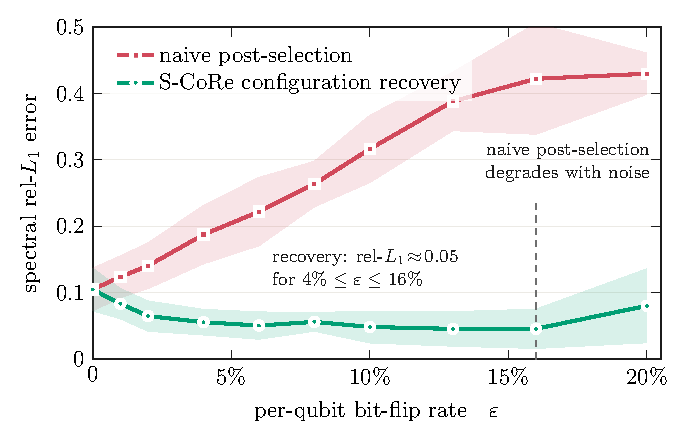
\includegraphics[width=0.7\linewidth]{figs/fig_noise_score.pdf}
\caption{\textbf{Noise robustness (synthetic per-qubit bit-flip channel, $L=6$).} Spectral
relative-$L_1$ error vs the per-qubit bit-flip rate $\varepsilon$, applied to bitstrings Born-sampled from
the exact distribution (this is a controlled classical simulation, not a device run). Naive
post-selection degrades steadily, whereas S-CoRe self-consistent configuration recovery, applied to the
same corrupted bitstrings, keeps the error near $0.05$ for $4\%\le\varepsilon\le16\%$ (periodic Hubbard
ring, $U/t=4$; seed-averaged over $6$ seeds at $6000$ shots each; bands $=\pm1$ s.d.\ across seeds). At
$\varepsilon=0$ the two arms coincide at $0.105$, about twice the acceptance threshold $0.05$ of the
resource scan, and the recovered error at finite $\varepsilon$ falls below that noiseless value; that
second comparison is not used here (Sec.~\ref{sec:scope:hw}): it is decided by the size of the recovered
subspace, which this sweep does not record.}\label{fig:noise}\end{figure*}
